\documentclass[11pt]{amsart}
\usepackage[a4paper,margin=1in]{geometry}
\usepackage{amsmath,amssymb,amsthm}
\usepackage{tikz}
\usepackage{booktabs}
\usepackage[hidelinks]{hyperref}
\newcommand{\doi}[1]{doi:\href{https://doi.org/#1}{#1}}

\newtheorem{thm}{Theorem}[section]
\newtheorem{lemma}[thm]{Lemma}
\newtheorem{prop}[thm]{Proposition}
\newtheorem{cor}[thm]{Corollary}
\newtheorem{conj}[thm]{Conjecture}
\theoremstyle{definition}
\newtheorem{definition}[thm]{Definition}
\newtheorem{remark}[thm]{Remark}

\newcommand{\sig}{\sigma}
\DeclareMathOperator{\br}{br}

\title[Remoteness minimisers with three branch vertices]{A tree of given segment sequence whose remoteness minimisers all have three branch vertices}
\author{Vamshi Jandhyala}
\address{London, United Kingdom}
\date{Preprint, version 1, 23 November 2026. Not peer reviewed.}
\subjclass[2020]{05C05, 05C12, 05C35}
\keywords{remoteness, transmission, segment sequence, extremal trees, outpost}

\begin{document}

\begin{abstract}
The remoteness of a connected graph is the largest average distance from a vertex to all others. Allie, du Preez,
Hefty and Mafunda conjectured that among all trees with a given segment sequence, a tree of minimum remoteness is
starlike or has exactly two branch vertices. We show that this fails. For the segment sequence
$(53,23,21,9,9,9,1,1,1,1,1,1)$ every tree of minimum remoteness has exactly three branch vertices, and the same holds
after multiplying every length by any positive integer. The obstruction is arithmetic: a tree with at most two branch
vertices must split the short segments into two groups of prescribed total, and no subset of the short segments has
that total. We also prove that the conjecture holds for every segment sequence of the form $(L,p,h,\dots,h)$, the shape
the authors identified as the most likely source of a counterexample.
\end{abstract}

\maketitle

\section{Introduction}

Suppose we are handed a list of path lengths and must glue the paths together at their ends into a single tree, so
that no vertex ends up far from the others on average. Allie, du Preez, Hefty and Mafunda conjectured that the best
arrangement never needs more than two junction points. We show that three can be necessary.

Let $T$ be a tree on $n\ge2$ vertices. The \emph{transmission} of a vertex $v$ is $\sig(v)=\sum_{u}d(v,u)$, and the
\emph{remoteness} of $T$ is $\rho(T)=\max_v \sig(v)/(n-1)$, the largest average distance from a vertex to the
others~\cite{AH}. A \emph{segment} of $T$ is a maximal path whose internal vertices have degree~$2$; its ends are
leaves or \emph{branch vertices} (vertices of degree at least~$3$). Figure~\ref{fig:T} shows a tree with twelve
segments and three branch vertices. The lengths of the segments, in non-increasing
order, form the \emph{segment sequence} of $T$, and $T$ is then called a $D$-tree. A tree with exactly $h$ branch
vertices is a $(\Delta,h)$-tree, and it is \emph{starlike} when $h=1$.

Allie, du Preez, Hefty and Mafunda~\cite{ADHM} determined the $D$-trees of minimum proximity and maximum remoteness,
and showed that the $D$-tree of minimum remoteness is sometimes starlike and sometimes has two branch vertices. They
proposed the following.

\begin{conj}[{\cite[Conjecture~4.4]{ADHM}}]\label{conj}
For every segment sequence $D$, the $D$-tree with minimum remoteness is starlike or a $(\Delta,2)$-$D$-tree.
\end{conj}

The concluding section of~\cite{ADHM} states it for ``a'' $D$-tree of minimum remoteness; Theorem~\ref{thm:main}
below refutes it in either reading. Before stating it they searched by computer, without success, for a counterexample among sequences in which the
longest segment is much longer than the second, which is much longer than all the others, all equal~\cite[\S4]{ADHM}.
Their concluding section asks whether a tree with three or more branch vertices can ever minimise
remoteness~\cite[\S7]{ADHM}. We answer that question.

\begin{thm}\label{thm:main}
Let $D=(53,23,21,9,9,9,1,1,1,1,1,1)$. Every $D$-tree of minimum remoteness has exactly three branch vertices. For
every integer $s\ge1$ the same holds for the sequence $sD$ obtained by multiplying every length by $s$.
\end{thm}

The tree that attains the minimum is drawn in Figure~\ref{fig:T}. Section~\ref{sec:cx} proves by hand that it beats
every starlike tree and every tree with two branch vertices; that alone refutes Conjecture~\ref{conj}. The statement
that no tree with four or five branch vertices does better is a finite computation, described in
Proposition~\ref{prop:all}.

The shape searched in~\cite{ADHM} cannot produce a counterexample.

\begin{thm}\label{thm:family}
Let $D=(L,p,h,\dots,h)$ with $m\ge1$ copies of $h$ and $L\ge p\ge h\ge1$. Then every $D$-tree of minimum remoteness
is starlike or has two branch vertices.
\end{thm}

In the counterexample six segments are longer than the shortest one; Theorem~\ref{thm:family} shows that two never
suffice. The cases in between, and the fewest segments in a counterexample, are open (Remark~\ref{rem:open}).

\begin{figure}[t]
\centering
\begin{tikzpicture}[scale=1,every node/.style={font=\small}]
  \coordinate (a) at (0,0); \coordinate (b) at (5.3,0); \coordinate (c) at (7.6,0);
  \draw[thick] (a) -- node[above]{$53$} (b) -- node[above]{$23$} (c);
  \foreach \ang/\lab in {150/9,180/9,210/9}{\draw[thick] (a) -- ++(\ang:0.9) node[left]{\lab};}
  \draw[thick] (b) -- ++(270:2.1) node[below]{$21$};
  \foreach \ang in {-50,-30,-10,10,30,50}{\draw[thick] (c) -- ++(\ang:0.45);}
  \node at (8.55,0) {$1^6$};
  \foreach \p in {a,b,c}{\fill (\p) circle (1.8pt);}
  \node[below right] at (a) {$x$}; \node[above right] at (b) {$y$}; \node[above] at (c) {$z$};
\end{tikzpicture}
\caption{The tree $T$ of Theorem~\ref{thm:main}, drawn with segments as edges labelled by their lengths. Its branch
vertices are $x$, $y$, $z$; $x$ carries three pendant segments of length $9$, $y$ one of length $21$, and $z$ six of
length $1$.}
\label{fig:T}
\end{figure}

\section{Transmission measured through segments}\label{sec:id}

Fix a $D$-tree $T$ with segments $S_1,\dots,S_k$ of lengths $\ell_1,\dots,\ell_k$. Write
\[
N=\sum_{i}\ell_i=n-1,\qquad Q=\sum_i\binom{\ell_i+1}{2},\qquad f(t)=t(N-t).
\]
Both $N$ and $Q$ depend only on $D$. For a vertex $v$ and a segment $S$ let $d(v,S)$ be the distance from $v$ to the
nearer end of~$S$, and put
\[
F(v)=\sum_i \ell_i\, d(v,S_i).
\]

\begin{lemma}\label{lem:id}
For every leaf or branch vertex $v$ of $T$, $\sig(v)=Q+F(v)$.
\end{lemma}

\begin{proof}
Since $v$ is an end of every segment containing it, we may assign to each segment $S$ the $\ell_S$ vertices of $S$
other than its end nearer to $v$. These sets
partition $V(T)\setminus\{v\}$, and the vertices assigned to $S$ lie at distances
$d(v,S)+1,\dots,d(v,S)+\ell_S$ from $v$. Their sum is $\ell_S\,d(v,S)+\binom{\ell_S+1}{2}$.
\end{proof}

\begin{lemma}[{\cite[Observation~2.7]{ADHM}}]\label{lem:leaf}
The maximum transmission of a tree is attained only at leaves. Consequently
$\rho(T)=\bigl(Q+C(T)\bigr)/N$ with $C(T)=\max\{F(x): x \text{ a leaf of } T\}$, and minimising $\rho$ over $D$-trees
is the same as minimising~$C$.
\end{lemma}

\begin{proof}
We recall the short argument. Let $v$ be a vertex that is not a leaf. Since $v$ has at least two neighbours, some component of $T-v$ has at most
$(n-1)/2$ vertices; let it have $s<n/2$ vertices, and let $w$ be the neighbour of $v$ in it. Moving from $v$ to $w$
brings $s$ vertices one step closer and takes the other $n-s$ one step further away, so
$\sig(w)-\sig(v)=n-2s>0$.
\end{proof}

When $x$ is the leaf of a pendant segment of length $a$ attached at a branch vertex $w$, every other segment is at
distance $a+d(w,S)$ from $x$, so
\begin{equation}\label{eq:leafvalue}
F(x)=f(a)+\Phi(w),\qquad \Phi(w)=\sum_i\ell_i\,d(w,S_i).
\end{equation}
In particular $F(x)\ge f(a)$. For two segments of lengths $a\ge b$ we have $a+b\le N$, hence
\begin{equation}\label{eq:fmono}
f(a)-f(b)=(a-b)(N-a-b)\ge0 .
\end{equation}

\begin{lemma}\label{lem:R}
Let $k\ge3$ and let $L=\ell_1$ be a longest segment length and put $D'=D\setminus\{L\}$ (one copy removed). The minimum of $C$ over
starlike $D$-trees and $(\Delta,2)$-$D$-trees is
\[
R(D)=\min\Bigl\{f(L),\ \min_{A\sqcup B=D',\ |A|,|B|\ge2}\ \max\bigl\{f(\max A)+L\textstyle\sum B,\ f(\max B)+L\sum A\bigr\}\Bigr\},
\]
where the inner minimum runs over the splittings of the multiset $D'$ into two parts of size at least~$2$, and is
$+\infty$ when there are none (as for $k\le4$).
\end{lemma}

\begin{proof}
In a starlike tree $\Phi$ vanishes at the centre, so by~\eqref{eq:leafvalue} and~\eqref{eq:fmono} its value is
$f(L)$. A tree with two branch vertices $u,v$ consists of a segment of some length $b$ joining them, with multisets
$A$ and $B$ of pendant lengths at $u$ and $v$, each of size at least $2$. Here $\Phi(u)=b\sum B$ and
$\Phi(v)=b\sum A$, so by~\eqref{eq:leafvalue} and~\eqref{eq:fmono} its value is
$\max\{f(\max A)+b\sum B,\ f(\max B)+b\sum A\}$. If $b=L$ this is one of the candidates in $R(D)$. If $b<L$ then a
segment of length $L$ is pendant and $C\ge f(L)$.
\end{proof}

\section{The counterexample}\label{sec:cx}

From now on $D=(53,23,21,9,9,9,1,1,1,1,1,1)$, so that $N=130$, $Q=2079$ and $f(t)=t(130-t)$. Let $T$ be the tree of
Figure~\ref{fig:T}.

\begin{lemma}\label{lem:T}
$C(T)=3883$.
\end{lemma}

\begin{proof}
By~\eqref{eq:leafvalue} each leaf value is $f(a)+\Phi(w)$, and
\begin{align*}
\Phi(x)&=53\,(21+23)+(53+23)\cdot6=2788, & f(9)+\Phi(x)&=1089+2788=3877,\\
\Phi(y)&=53\cdot27+23\cdot6=1569, & f(21)+\Phi(y)&=2289+1569=3858,\\
\Phi(z)&=23\,(21+53)+(23+53)\cdot27=3754, & f(1)+\Phi(z)&=129+3754=3883. \qedhere
\end{align*}
\end{proof}

\begin{lemma}\label{lem:RD}
$R(D)=3892$.
\end{lemma}

\begin{proof}
Here $f(L)=f(53)=4081$, and the splitting $A=\{23,21,1,1,1,1,1,1\}$, $B=\{9,9,9\}$ has value
$\max\{f(23)+53\cdot27,\ f(9)+53\cdot50\}=\max\{3892,3739\}=3892$. Suppose some splitting $A\sqcup B$ of
$D'=\{23,21,9,9,9,1^6\}$, whose total is $77$, had value at most $3891$; by symmetry $23\in A$. Then
$f(23)+53\sum B=2461+53\sum B\le3891$ forces $\sum B\le26$, so $\sum A\ge51$, and
$f(\max B)+53\sum A\le3891$ forces $f(\max B)\le3891-53\cdot51=1188<f(10)$. Hence $\max B\le9$, so
$B\subseteq\{9,9,9,1^6\}$. If $\max B=9$ the second condition reads $53(77-\sum B)\le2802$, that is $\sum B\ge25$; so
$\sum B\in\{25,26\}$. But a sum $9j+i$ with $1\le j\le3$ and $0\le i\le6$ takes the values
$9,\dots,15,18,\dots,24,27,\dots,33$ and misses $25$ and $26$. If $\max B=1$ the second condition reads
$53(77-\sum B)\le3762$, that is $\sum B\ge7$, while $B$ has at most six ones. Both cases are impossible.
\end{proof}

By Lemmas~\ref{lem:leaf}, \ref{lem:R}, \ref{lem:T} and~\ref{lem:RD}, the tree $T$ has smaller remoteness than every
starlike $D$-tree and every $(\Delta,2)$-$D$-tree:
\[
\rho(T)=\frac{2079+3883}{130}=\frac{5962}{130}<\frac{5971}{130}=\frac{2079+R(D)}{130}.
\]
So no $D$-tree of minimum remoteness is starlike or has two branch vertices, and Conjecture~\ref{conj} fails.

The proof of Lemma~\ref{lem:RD} shows where the two-branch trees lose (Figure~\ref{fig:mech}). The best of them puts $\{9,9,9\}$ at one end of
the long segment and everything else at the other, and its worst leaf is the end of the $23$-segment. Improving it
means moving short segments to the $\{9,9,9\}$ side until their total is $25$ or $26$, and the short segments cannot
make that total. The tree $T$ avoids the problem by not splitting at all: it hangs the six unit segments beyond the end
of the $23$-segment, which turns that segment into an internal one and lowers the worst leaf value from $3892$ to
$3883$.

\begin{figure}[t]
\centering
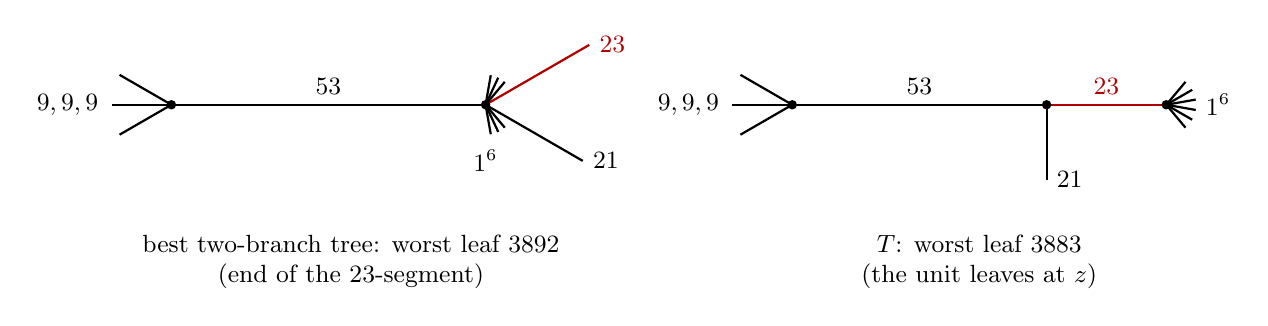
\begin{tikzpicture}[scale=0.95,every node/.style={font=\small}]
  % left: best two-branch tree
  \begin{scope}
    \coordinate (u) at (0,0); \coordinate (v) at (4.2,0);
    \draw[thick] (u) -- node[above]{$53$} (v);
    \foreach \ang in {150,180,210}{\draw[thick] (u) -- ++(\ang:0.8);}
    \node[left] at (-0.85,0) {$9,9,9$};
    \draw[thick,red!70!black] (v) -- ++(30:1.6) node[right]{$23$};
    \draw[thick] (v) -- ++(-30:1.5) node[right]{$21$};
    \foreach \ang in {-80,-65,-50,50,65,80}{\draw[thick] (v) -- ++(\ang:0.4);}
    \node at (4.2,-0.75) {$1^6$};
    \fill (u) circle (1.8pt); \fill (v) circle (1.8pt);
    \node[align=center] at (2.4,-2.1) {best two-branch tree: worst leaf $3892$\\(end of the $23$-segment)};
  \end{scope}
  % right: T
  \begin{scope}[xshift=8.3cm]
    \coordinate (a) at (0,0); \coordinate (b) at (3.4,0); \coordinate (c) at (5.0,0);
    \draw[thick] (a) -- node[above]{$53$} (b);
    \draw[thick,red!70!black] (b) -- node[above]{$23$} (c);
    \foreach \ang in {150,180,210}{\draw[thick] (a) -- ++(\ang:0.8);}
    \node[left] at (-0.85,0) {$9,9,9$};
    \draw[thick] (b) -- ++(270:1.0) node[right]{$21$};
    \foreach \ang in {-50,-30,-10,10,30,50}{\draw[thick] (c) -- ++(\ang:0.4);}
    \node[right] at (5.4,0) {$1^6$};
    \foreach \p in {a,b,c}{\fill (\p) circle (1.8pt);}
    \node[align=center] at (2.5,-2.1) {$T$: worst leaf $3883$\\(the unit leaves at $z$)};
  \end{scope}
\end{tikzpicture}
\caption{The mechanism. Left: the best tree with two branch vertices; rebalancing it would need short segments of
total $25$ or $26$ on the $\{9,9,9\}$ side, and $\{9,9,9,1^6\}$ has no such subset. Right: $T$ moves the six unit
segments to the far end of the $23$-segment instead, and every leaf value drops below $3892$.}
\label{fig:mech}
\end{figure}

\begin{prop}\label{prop:all}
For $D=(53,23,21,9,9,9,1^6)$, the minimum of $C$ over $D$-trees with exactly $h$ branch vertices is
\[
\begin{array}{c|ccccc}
h&1&2&3&4&5\\\hline
\min C&4081&3892&3883&3896&3924
\end{array}
\]
and no $D$-tree has more than five branch vertices. In particular $T$ attains the minimum of $C$, and every $D$-tree
of minimum remoteness has exactly three branch vertices.
\end{prop}

\begin{proof}
A tree with $k$ segments and $h$ branch vertices has at least $h+2$ leaves and $k=\#\text{leaves}+h-1$ segments, so
$h\le(k-1)/2=5.5$. The table is a finite computation: every one of the $42$ series-reduced trees with $12$ edges,
with every one of the $110{,}880$ distinct assignments of the lengths in $D$ to its edges, evaluated with
Lemma~\ref{lem:id}. Two programs written independently, sharing no code, produce the same table, and a third
confirms the rows $h\le2$ and the value of $T$ by breadth-first search on the subdivided trees; they are described in
Section~\ref{sec:data}. The values for $h=1,2$ also follow from Lemmas~\ref{lem:R} and~\ref{lem:RD}, and
Lemma~\ref{lem:T} shows that $3883$ is attained for $h=3$; that no tree with three branch vertices does better rests
on the computation.
\end{proof}

\begin{proof}[Proof of Theorem~\ref{thm:main}]
The case $s=1$ is Proposition~\ref{prop:all}. Multiplying every length by $s$ maps $D$-trees bijectively to
$sD$-trees with the same branch vertices, and multiplies every $d(v,S)$ and every $\ell_i$ by $s$ when $v$ is a branch
vertex or a leaf. So $F$ at each leaf, and hence $C$, is multiplied by $s^2$, while $Q$ is the same for all
$sD$-trees. By Lemma~\ref{lem:leaf} the order of the $sD$-trees by remoteness is the order of the $D$-trees by~$C$.
\end{proof}

\begin{remark}\label{rem:second}
The first counterexample we found is larger. Take
\[
D=(133,49,46,42,32,29,28,25,1^{11}).
\]
The tree whose branch vertices form a path $x$--$y$--$z$ with segments $133$ and $49$, carrying pendant segments $\{32,29,28,25\}$ at $x$,
$\{46,42\}$ at $y$ and eleven unit segments at $z$, has maximum transmission $45796$; the best starlike or
$(\Delta,2)$-$D$-tree has $45941$. The mechanism is the same.
\end{remark}

\begin{remark}\label{rem:open}
Exhaustive searches over all $D$-trees with $k\le7$ segments of length at most $10$, $k=8$ with lengths at most $9$,
$k=9$ with lengths at most $5$ and $k=10$ with lengths at most $3$ found no counterexample; the programs and their logs are in the archive. We do not know the least $k$ for which
Conjecture~\ref{conj} fails, nor whether it can fail when only three, four or five segments are longer than the
shortest; Theorem~\ref{thm:family} settles two, and $D$ has six.
\end{remark}

\section{Sequences with two long segments}\label{sec:family}

The strategy is to simplify an arbitrary $D$-tree without increasing its remoteness until it has at most three
branch vertices, and then to beat the three-branch survivors directly. Short internal segments can always be made
pendant at a strict gain (Lemmas~\ref{lem:star} and~\ref{lem:prune}); what remains has only the two long segments as
internal ones. For such a tree the two end leaves have values summing to $f(L)+f(p)+2f(h)$, and a two-branch tree
with a well-chosen split of the $h$-segments comes within $Lh/2$ of the average of the same three terms. Since
$f(h)>Lh$, the average of the two leaves is already larger (Lemma~\ref{lem:three}). The equal lengths are what make
the split fine enough; the counterexample of Section~\ref{sec:cx} is exactly a case where they are not.

We use the starring operation of~\cite[Definition~2.8]{ADHM}: for a non-pendant segment $S$ with ends $u,v$, remove
$S$, identify $u$ and $v$ into one vertex $w$, and attach at $w$ a pendant segment of the same length. It preserves
the segment sequence and removes one branch vertex.

\begin{lemma}[{\cite[Lemma~4.1]{ADHM}}]\label{lem:star}
If a pendant segment of length $\ell_i$ is adjacent to a non-pendant segment $S_j$ with $\ell_i\ge\ell_j$, then
starring $S_j$ strictly decreases the remoteness.
\end{lemma}

For the rest of this section $D=(L,p,h^m)$ with $L\ge p\ge h\ge1$ and $m\ge1$.

\begin{lemma}\label{lem:prune}
If a $D$-tree has a non-pendant segment of length $h$, then some non-pendant segment of length $h$ is adjacent to a
pendant segment.
\end{lemma}

\begin{proof}
Let $K$ be the tree formed by the branch vertices, joined when a non-pendant segment joins them. Let $J$ be a
component, with at least one edge, of the subgraph of $K$ formed by the segments of length $h$, and let $u\ne v$ be two
leaves of $J$. If neither $u$ nor $v$ lies on a pendant segment, each has degree at least $3$ in $K$ and degree $1$ in
$J$, so each meets at least two non-pendant segments of length other than $h$. These are at least three distinct
segments, since only a segment joining $u$ and $v$ could be counted twice, and it would close a cycle with the path from
$u$ to $v$ in $J$. But only two segments of $D$ have length other than~$h$. So $u$ or $v$ carries a pendant segment,
whose length is at least $h$, adjacent to its segment of length $h$ in~$J$.
\end{proof}

\begin{lemma}\label{lem:three}
Suppose $p>h$ and the non-pendant segments of a $D$-tree $T$ are exactly the segments of lengths $L$ and $p$. Then
$C(T)>R(D)$.
\end{lemma}

\begin{proof}
The branch vertices form a path $x$--$y$--$z$ with the $L$-segment from $x$ to $y$ and the $p$-segment from $y$ to $z$;
every pendant segment has length $h$. Let $x,y,z$ carry $a,b,c$ of them, so $a,c\ge2$, $b\ge1$ and $a+b+c=m$. Here
$N=L+p+mh$. By~\eqref{eq:leafvalue} the leaves at $x$ and at $z$ have values
\[
X=f(h)+L\bigl(p+(b+c)h\bigr)+pch,\qquad Z=f(h)+p\bigl(L+(a+b)h\bigr)+Lah,
\]
and a direct expansion gives $X+Z=2f(h)+2Lp+(L+p)mh=f(L)+f(p)+2f(h)$. Hence
\begin{equation}\label{eq:avg}
C(T)\ge\tfrac12(X+Z)=H_0+\tfrac12f(h),\qquad H_0=\tfrac12\bigl(f(L)+f(p)+f(h)\bigr).
\end{equation}
Now consider the two-branch trees with the $L$-segment between the branch vertices, $p$ and $m-r$ segments of length
$h$ at one end and $r$ at the other, $2\le r\le m-1$. By Lemma~\ref{lem:R} their value is
$H(r)=\max\{f(p)+Lrh,\ f(h)+L(p+(m-r)h)\}$. Extend $H$ to real $r$. The two affine pieces have slopes $\pm Lh$ and
cross at
\[
r_0=\frac{f(h)+f(L)-f(p)}{2Lh}=1+\frac{(m-1)(L-p+h)}{2L}
\]
with common value $H_0$. Since $h\le p\le L$ we get $1<r_0\le(m+1)/2\le m-1$, using $m=a+b+c\ge5$. Let $j$ be an
integer in $[1,m-1]$ nearest to $r_0$, so $H(j)=H_0+Lh\,|j-r_0|\le H_0+Lh/2$. If $j\ge2$ then $R(D)\le H(j)$. If
$j=1$, then $H(1)\ge f(h)+L(p+(m-1)h)=f(L)+f(h)-Lh>f(L)\ge R(D)$, because $f(h)=h(N-h)>Lh$. Either way
$R(D)\le H_0+Lh/2<H_0+f(h)/2\le C(T)$, again by $f(h)>Lh$.
\end{proof}

\begin{proof}[Proof of Theorem~\ref{thm:family}]
Let $T$ be any $D$-tree. While $T$ has a non-pendant segment of length $h$, Lemma~\ref{lem:prune} provides one adjacent
to a pendant segment of length at least $h$, and Lemma~\ref{lem:star} lets us star it, strictly decreasing the
remoteness. Starring makes the segment pendant and changes no other segment, so this stops after finitely many steps
with a tree $T_0$ whose non-pendant segments all have length greater than $h$. There are at most two of those, so $T_0$
has at most three branch vertices.

If $T_0$ is starlike, $C(T_0)=f(L)\ge R(D)$. If it has two branch vertices, $C(T_0)\ge R(D)$ by Lemma~\ref{lem:R}. If
it has three, its non-pendant segments are the two segments longer than $h$, so $p>h$ and $C(T_0)>R(D)$ by
Lemma~\ref{lem:three}. In all cases $C(T)\ge C(T_0)\ge R(D)$, and by Lemma~\ref{lem:R} the value $R(D)$ is attained by
a starlike or two-branch $D$-tree. If $T$ has at least three branch vertices, then either some starring was applied,
so $C(T)>C(T_0)\ge R(D)$, or $T=T_0$ has three branch vertices and $C(T)>R(D)$. So no tree with three or more branch
vertices has minimum remoteness.
\end{proof}

The case $p=h$ is the family $(bh,h,\dots,h)$ of~\cite[Theorem~4.2 and Corollary~4.3]{ADHM}, which give sufficient
conditions for each of the two outcomes; Theorem~\ref{thm:family} together with Lemma~\ref{lem:R} gives the minimum
value for every such sequence.

\section{Data, code and the use of AI tools}\label{sec:data}

The accompanying archive contains three programs that share no code. The first program, \texttt{true\_min.py}, enumerates the
series-reduced trees with $k$ edges and all distinct length assignments, and evaluates $C$ through the quadratic forms of
Lemma~\ref{lem:id}; it produces the table of Proposition~\ref{prop:all}. The second, \texttt{recheck\_table.py},
generates the skeletons afresh (\texttt{networkx}, $42$ trees) and computes each $F(x)$ from the edges on the path
from $x$ to the nearer end of each segment; it reproduces the table. The third, \texttt{verify\_exhaustive.py},
builds the subdivided trees explicitly and runs breadth-first search from every leaf, for $T$, for the starlike tree
and for every $(\Delta,2)$-$D$-tree with every choice of the joining segment; it confirms the maximum transmissions
$5962$, $6160$ and $5971$. Each program stops with an error if its results differ from the values stated here.
The searches of Remark~\ref{rem:open} are archived with their logs. The archive is deposited at Zenodo,
\doi{10.5281/zenodo.24483605}, and is identical to the folder \texttt{remoteness-three-branch-trees} of
\url{https://github.com/jvvk/mathematics} at tag \texttt{remoteness-three-branch-trees-v1}.

Parts of the argument are formalised in Lean~4 with Mathlib, on Mathlib's graph distance: Lemma~\ref{lem:RD} over
every splitting of $D'$; Lemma~\ref{lem:three} for all admissible parameters; Lemma~\ref{lem:prune}; and, for trees
built from a path with pendant paths attached (which include $T$, every starlike $D$-tree and every
$(\Delta,2)$-$D$-tree), the distance formula, Lemma~\ref{lem:id} at the leaves, Lemma~\ref{lem:leaf}, Lemma~\ref{lem:T}, the maximum
transmission of $T$ ($5962$) and the lower bound $5971$ for every starlike or $(\Delta,2)$-$D$-tree, and the branch
vertices of each. Not formalised: Lemma~\ref{lem:star}, which we cite; the identification of an arbitrary tree with at
most two branch vertices with such a path-with-pendants tree; and the rows $h=3,4,5$ of Proposition~\ref{prop:all},
which rest on the computation.

The author used AI tools: Claude (Anthropic) found the counterexample, by a search directed at the arithmetic
obstruction described after Lemma~\ref{lem:RD}, and wrote the code, the Lean formalisation and the text; Codex (OpenAI) found the proof of
Theorem~\ref{thm:family}, identified in a failed proof attempt the subset-sum obstruction that directed the search, and
independently rechecked the counterexample of Remark~\ref{rem:second} with its own code.
The author is responsible for the content.

\begin{thebibliography}{9}

\bibitem{ADHM}
I.~Allie, B.~du~Preez, Z.~Hefty and S.~Mafunda, \emph{Proximity and remoteness in trees with given segment sequence},
arXiv:2611.27685v1 [math.CO], 20 November 2026, \url{https://arxiv.org/abs/2611.27685} (accessed 23 November 2026).

\bibitem{AH}
M.~Aouchiche and P.~Hansen, \emph{Proximity and remoteness in graphs: results and conjectures}, Networks \textbf{58}
(2011), no.~2, 95--102, \doi{10.1002/net.20450}.

\end{thebibliography}

\end{document}
